\documentclass[11pt,journal,compsoc, onecolumn]{IEEEtran}
\usepackage{listings}
\usepackage{color}


\definecolor{mygreen}{rgb}{0,0.6,0}
\definecolor{mygray}{rgb}{0.5,0.5,0.5}
\definecolor{myred}{rgb}{0.6,0,0}



\lstset{ %
  backgroundcolor=\color{white},   % choose the background color; you must add \usepackage{color} or \usepackage{xcolor}
  basicstyle=\normalsize,        % the size of the fonts that are used for the code
  breakatwhitespace=false,         % sets if automatic breaks should only happen at whitespace
  breaklines=true,                 % sets automatic line breaking
  captionpos=b,                    % sets the caption-position to bottom
  commentstyle=\color{mygreen},    % comment style
  deletekeywords={...},            % if you want to delete keywords from the given language
  escapeinside={\%*}{*)},          % if you want to add LaTeX within your code
  extendedchars=true,              % lets you use non-ASCII characters; for 8-bits encodings only, does not work with UTF-8
  frame=single,                    % adds a frame around the code
  keepspaces=true,                 % keeps spaces in text, useful for keeping indentation of code (possibly needs columns=flexible)
  keywordstyle=\color{mygreen},       % keyword style
  language=C,                 % the language of the code
  otherkeywords={*,...},            % if you want to add more keywords to the set
  numbers=left,                    % where to put the line-numbers; possible values are (none, left, right)
  numbersep=5pt,                   % how far the line-numbers are from the code
  numberstyle=\tiny\color{mygray}, % the style that is used for the line-numbers
  rulecolor=\color{black},         % if not set, the frame-color may be changed on line-breaks within not-black text (e.g. comments (green here))
  showspaces=false,                % show spaces everywhere adding particular underscores; it overrides 'showstringspaces'
  showstringspaces=false,          % underline spaces within strings only
  showtabs=false,                  % show tabs within strings adding particular underscores
  stepnumber=1,                    % the step between two line-numbers. If it's 1, each line will be numbered
  stringstyle=\color{myred},     % string literal style
  tabsize=2,                       % sets default tabsize to 2 spaces
  title=\lstname                   % show the filename of files included with \lstinputlisting; also try caption instead of title
}
%
% If IEEEtran.cls has not been installed into the LaTeX system files,
% manually specify the path to it like:
% \documentclass[12pt,journal,compsoc]{../sty/IEEEtran}





% Some very useful LaTeX packages include:
% (uncomment the ones you want to load)


% *** MISC UTILITY PACKAGES ***
%
\usepackage{ifpdf}
% Heiko Oberdiek's ifpdf.sty is very useful if you need conditional
% compilation based on whether the output is pdf or dvi.
% usage:
% \ifpdf
%   % pdf code
% \else
%   % dvi code
% \fi
% The latest version of ifpdf.sty can be obtained from:
% http://www.ctan.org/tex-archive/macros/latex/contrib/oberdiek/
% Also, note that IEEEtran.cls V1.7 and later provides a builtin
% \ifCLASSINFOpdf conditional that works the same way.
% When switching from latex to pdflatex and vice-versa, the compiler may
% have to be run twice to clear warning/error messages.






% *** CITATION PACKAGES ***
%
\ifCLASSOPTIONcompsoc
  % IEEE Computer Society needs nocompress option
  % requires cite.sty v4.0 or later (November 2003)
   \usepackage[nocompress]{cite}
\else
  % normal IEEE
   \usepackage{cite}
\fi
% cite.sty was written by Donald Arseneau
% V1.6 and later of IEEEtran pre-defines the format of the cite.sty package
% \cite{} output to follow that of IEEE. Loading the cite package will
% result in citation numbers being automatically sorted and properly
% "compressed/ranged". e.g., [1], [9], [2], [7], [5], [6] without using
% cite.sty will become [1], [2], [5]--[7], [9] using cite.sty. cite.sty's
% \cite will automatically add leading space, if needed. Use cite.sty's
% noadjust option (cite.sty V3.8 and later) if you want to turn this off
% such as if a citation ever needs to be enclosed in parenthesis.
% cite.sty is already installed on most LaTeX systems. Be sure and use
% version 4.0 (2003-05-27) and later if using hyperref.sty. cite.sty does
% not currently provide for hyperlinked citations.
% The latest version can be obtained at:
% http://www.ctan.org/tex-archive/macros/latex/contrib/cite/
% The documentation is contained in the cite.sty file itself.
%
% Note that some packages require special options to format as the Computer
% Society requires. In particular, Computer Society  papers do not use
% compressed citation ranges as is done in typical IEEE papers
% (e.g., [1]-[4]). Instead, they list every citation separately in order
% (e.g., [1], [2], [3], [4]). To get the latter we need to load the cite
% package with the nocompress option which is supported by cite.sty v4.0
% and later. Note also the use of a CLASSOPTION conditional provided by
% IEEEtran.cls V1.7 and later.



\usepackage{graphicx}

% *** GRAPHICS RELATED PACKAGES ***
%
\ifCLASSINFOpdf
  % \usepackage[pdftex]{graphicx}
  % declare the path(s) where your graphic files are
  % \graphicspath{{../pdf/}{../jpeg/}}
  % and their extensions so you won't have to specify these with
  % every instance of \includegraphics
  % \DeclareGraphicsExtensions{.pdf,.jpeg,.png}
\else
  % or other class option (dvipsone, dvipdf, if not using dvips). graphicx
  % will default to the driver specified in the system graphics.cfg if no
  % driver is specified.
  % \usepackage[dvips]{graphicx}
  % declare the path(s) where your graphic files are
  % \graphicspath{{../eps/}}
  % and their extensions so you won't have to specify these with
  % every instance of \includegraphics
  % \DeclareGraphicsExtensions{.eps}
\fi
% graphicx was written by David Carlisle and Sebastian Rahtz. It is
% required if you want graphics, photos, etc. graphicx.sty is already
% installed on most LaTeX systems. The latest version and documentation
% can be obtained at: 
% http://www.ctan.org/tex-archive/macros/latex/required/graphics/
% Another good source of documentation is "Using Imported Graphics in
% LaTeX2e" by Keith Reckdahl which can be found at:
% http://www.ctan.org/tex-archive/info/epslatex/
%
% latex, and pdflatex in dvi mode, support graphics in encapsulated
% postscript (.eps) format. pdflatex in pdf mode supports graphics
% in .pdf, .jpeg, .png and .mps (metapost) formats. Users should ensure
% that all non-photo figures use a vector format (.eps, .pdf, .mps) and
% not a bitmapped formats (.jpeg, .png). IEEE frowns on bitmapped formats
% which can result in "jaggedy"/blurry rendering of lines and letters as
% well as large increases in file sizes.
%
% You can find documentation about the pdfTeX application at:
% http://www.tug.org/applications/pdftex






% *** MATH PACKAGES ***
%
\usepackage[cmex10]{amsmath}
% A popular package from the American Mathematical Society that provides
% many useful and powerful commands for dealing with mathematics. If using
% it, be sure to load this package with the cmex10 option to ensure that
% only type 1 fonts will utilized at all point sizes. Without this option,
% it is possible that some math symbols, particularly those within
% footnotes, will be rendered in bitmap form which will result in a
% document that can not be IEEE Xplore compliant!
%
% Also, note that the amsmath package sets \interdisplaylinepenalty to 10000
% thus preventing page breaks from occurring within multiline equations. Use:
%\interdisplaylinepenalty=2500
% after loading amsmath to restore such page breaks as IEEEtran.cls normally
% does. amsmath.sty is already installed on most LaTeX systems. The latest
% version and documentation can be obtained at:
% http://www.ctan.org/tex-archive/macros/latex/required/amslatex/math/





% *** SPECIALIZED LIST PACKAGES ***
%
%\usepackage{algorithmic}
% algorithmic.sty was written by Peter Williams and Rogerio Brito.
% This package provides an algorithmic environment fo describing algorithms.
% You can use the algorithmic environment in-text or within a figure
% environment to provide for a floating algorithm. Do NOT use the algorithm
% floating environment provided by algorithm.sty (by the same authors) or
% algorithm2e.sty (by Christophe Fiorio) as IEEE does not use dedicated
% algorithm float types and packages that provide these will not provide
% correct IEEE style captions. The latest version and documentation of
% algorithmic.sty can be obtained at:
% http://www.ctan.org/tex-archive/macros/latex/contrib/algorithms/
% There is also a support site at:
% http://algorithms.berlios.de/index.html
% Also of interest may be the (relatively newer and more customizable)
% algorithmicx.sty package by Szasz Janos:
% http://www.ctan.org/tex-archive/macros/latex/contrib/algorithmicx/




% *** ALIGNMENT PACKAGES ***
%
%\usepackage{array}
% Frank Mittelbach's and David Carlisle's array.sty patches and improves
% the standard LaTeX2e array and tabular environments to provide better
% appearance and additional user controls. As the default LaTeX2e table
% generation code is lacking to the point of almost being broken with
% respect to the quality of the end results, all users are strongly
% advised to use an enhanced (at the very least that provided by array.sty)
% set of table tools. array.sty is already installed on most systems. The
% latest version and documentation can be obtained at:
% http://www.ctan.org/tex-archive/macros/latex/required/tools/


% IEEEtran contains the IEEEeqnarray family of commands that can be used to
% generate multiline equations as well as matrices, tables, etc., of high
% quality.




% *** SUBFIGURE PACKAGES ***
%\ifCLASSOPTIONcompsoc
%  \usepackage[caption=false,font=normalsize,labelfont=sf,textfont=sf]{subfig}
%\else
%  \usepackage[caption=false,font=footnotesize]{subfig}
%\fi
% subfig.sty, written by Steven Douglas Cochran, is the modern replacement
% for subfigure.sty, the latter of which is no longer maintained and is
% incompatible with some LaTeX packages including fixltx2e. However,
% subfig.sty requires and automatically loads Axel Sommerfeldt's caption.sty
% which will override IEEEtran.cls' handling of captions and this will result
% in non-IEEE style figure/table captions. To prevent this problem, be sure
% and invoke subfig.sty's "caption=false" package option (available since
% subfig.sty version 1.3, 2005/06/28) as this is will preserve IEEEtran.cls
% handling of captions.
% Note that the Computer Society format requires a larger sans serif font
% than the serif footnote size font used in traditional IEEE formatting
% and thus the need to invoke different subfig.sty package options depending
% on whether compsoc mode has been enabled.
%
% The latest version and documentation of subfig.sty can be obtained at:
% http://www.ctan.org/tex-archive/macros/latex/contrib/subfig/




% *** FLOAT PACKAGES ***
%
%\usepackage{fixltx2e}
% fixltx2e, the successor to the earlier fix2col.sty, was written by
% Frank Mittelbach and David Carlisle. This package corrects a few problems
% in the LaTeX2e kernel, the most notable of which is that in current
% LaTeX2e releases, the ordering of single and double column floats is not
% guaranteed to be preserved. Thus, an unpatched LaTeX2e can allow a
% single column figure to be placed prior to an earlier double column
% figure. The latest version and documentation can be found at:
% http://www.ctan.org/tex-archive/macros/latex/base/


%\usepackage{stfloats}
% stfloats.sty was written by Sigitas Tolusis. This package gives LaTeX2e
% the ability to do double column floats at the bottom of the page as well
% as the top. (e.g., "\begin{figure*}[!b]" is not normally possible in
% LaTeX2e). It also provides a command:
%\fnbelowfloat
% to enable the placement of footnotes below bottom floats (the standard
% LaTeX2e kernel puts them above bottom floats). This is an invasive package
% which rewrites many portions of the LaTeX2e float routines. It may not work
% with other packages that modify the LaTeX2e float routines. The latest
% version and documentation can be obtained at:
% http://www.ctan.org/tex-archive/macros/latex/contrib/sttools/
% Do not use the stfloats baselinefloat ability as IEEE does not allow
% \baselineskip to stretch. Authors submitting work to the IEEE should note
% that IEEE rarely uses double column equations and that authors should try
% to avoid such use. Do not be tempted to use the cuted.sty or midfloat.sty
% packages (also by Sigitas Tolusis) as IEEE does not format its papers in
% such ways.
% Do not attempt to use stfloats with fixltx2e as they are incompatible.
% Instead, use Morten Hogholm'a dblfloatfix which combines the features
% of both fixltx2e and stfloats:
%
% \usepackage{dblfloatfix}
% The latest version can be found at:
% http://www.ctan.org/tex-archive/macros/latex/contrib/dblfloatfix/




%\ifCLASSOPTIONcaptionsoff
%  \usepackage[nomarkers]{endfloat}
% \let\MYoriglatexcaption\caption
% \renewcommand{\caption}[2][\relax]{\MYoriglatexcaption[#2]{#2}}
%\fi
% endfloat.sty was written by James Darrell McCauley, Jeff Goldberg and 
% Axel Sommerfeldt. This package may be useful when used in conjunction with 
% IEEEtran.cls'  captionsoff option. Some IEEE journals/societies require that
% submissions have lists of figures/tables at the end of the paper and that
% figures/tables without any captions are placed on a page by themselves at
% the end of the document. If needed, the draftcls IEEEtran class option or
% \CLASSINPUTbaselinestretch interface can be used to increase the line
% spacing as well. Be sure and use the nomarkers option of endfloat to
% prevent endfloat from "marking" where the figures would have been placed
% in the text. The two hack lines of code above are a slight modification of
% that suggested by in the endfloat docs (section 8.4.1) to ensure that
% the full captions always appear in the list of figures/tables - even if
% the user used the short optional argument of \caption[]{}.
% IEEE papers do not typically make use of \caption[]'s optional argument,
% so this should not be an issue. A similar trick can be used to disable
% captions of packages such as subfig.sty that lack options to turn off
% the subcaptions:
% For subfig.sty:
% \let\MYorigsubfloat\subfloat
% \renewcommand{\subfloat}[2][\relax]{\MYorigsubfloat[]{#2}}
% However, the above trick will not work if both optional arguments of
% the \subfloat command are used. Furthermore, there needs to be a
% description of each subfigure *somewhere* and endfloat does not add
% subfigure captions to its list of figures. Thus, the best approach is to
% avoid the use of subfigure captions (many IEEE journals avoid them anyway)
% and instead reference/explain all the subfigures within the main caption.
% The latest version of endfloat.sty and its documentation can obtained at:
% http://www.ctan.org/tex-archive/macros/latex/contrib/endfloat/
%
% The IEEEtran \ifCLASSOPTIONcaptionsoff conditional can also be used
% later in the document, say, to conditionally put the References on a 
% page by themselves.




% *** PDF, URL AND HYPERLINK PACKAGES ***
%
\usepackage{url}
% url.sty was written by Donald Arseneau. It provides better support for
% handling and breaking URLs. url.sty is already installed on most LaTeX
% systems. The latest version and documentation can be obtained at:
% http://www.ctan.org/tex-archive/macros/latex/contrib/url/
% Basically, \url{my_url_here}.





% *** Do not adjust lengths that control margins, column widths, etc. ***
% *** Do not use packages that alter fonts (such as pslatex).         ***
% There should be no need to do such things with IEEEtran.cls V1.6 and later.
% (Unless specifically asked to do so by the journal or conference you plan
% to submit to, of course. )


% correct bad hyphenation here
\hyphenation{op-tical net-works semi-conduc-tor}


\begin{document}
\title{PhD. Qualification Report \\ \LARGE{\textbf{Can High-Level Synthesis Compete Against a Hand-Written Code in the Cryptographic Domain? \\ A Case Study \cite{sel}}} \\ Authors: \\ Ekawat Homsirikamol and Kris Gaj}

\author{Ryan Silva \\ Boston University \\ Department of Electrical and Computer Engineering \\ rjsilva@bu.edu
        % <-this % stops a space
%\IEEEcompsocitemizethanks{\IEEEcompsocthanksitem R. Silva is with the Department
%of Electrical and Computer Engineering, Boston University, Boston, 
%MA.\protect\\
% note need leading \protect in front of \\ to get a newline within \thanks as
% \\ is fragile and will error, could use \hfil\break instead.
%E-mail: ryan.jay.silva@gmail.com 
%}% <-this % stops an unwanted space
}

%\IEEEtitleabstractindextext{
%\begin{abstract}
%This is the master document. Abstracts for individual topics can be found in each section.
%\end{abstract}}

\maketitle


\IEEEdisplaynontitleabstractindextext
\IEEEpeerreviewmaketitle

\section{Introduction}
\IEEEPARstart{E}{ver-increasing} computational complexity creates situations in which the demands of pure software solutions bog down a general-purpose CPU to the point of impracticality. One mechanism used to mitigate such situations is through the use of hardware accelerators, i.e., offloading specific computational tasks to hardware. Developing hardware solutions to replace software comes with the trade-off of increased development time due to the introduction of hardware's inherent lower abstraction levels. This increased overhead can often be prohibitive, thus it has been a dream of hardware designers since the 1970s to create tools that reliably synthesize hardware using traditional software development techniques\cite{1}. This dream tool would complete a process known as High Level Synthesis (HLS).

In order to consider the dream realized, logic synthesis must operate reliably using an abstract, algorithmic level description of a circuit as the primary input specification\cite{mcfarland}. Unfortunately, due to reasons such as standardization\cite{ieee}, reliability\cite{tosun} and portability\cite{churtl}, the two most ubiquitous languages for constructing hardware descriptions (VHDL and Verilog) do not operate natively at the algorithmic level \cite{Harris+Harris}. This presents a problem: the most oft-used, best supported, languages for specifying synthesizable hardware do not behave like that of traditional compiled software. These two languages operate at a level of abstraction known as the Register-Transfer Level (RTL), which is one level of abstraction below that of the algorithmic level \cite{vahid}, and HLS seeks to bridge that gap.

The development of HLS tools is not the focus of Homsirikamol and Gaj's study, rather they seek to validate the state of the HLS dream by comparing the performance of hardware generated using an RTL circuit description to that of an algorithmic, HLS, specification. This report will explain the methodology used to conduct the case study and evaluate its conclusions based on alternative methods of comparison, ultimately presenting a more complete picture of whether HLS is a dream-come-true.


\section{Background}
%The term ``synthesis'' can be used to reference either the process of traversing abstraction levels in hardware design or as the process of mapping a behavioral description into a structural layout. The former definition is accomplished by implementing a description found at a higher level of abstraction using only methods found in the lower level, and serves as the focus of this review\cite{churtl}. The two most ubiquitous languages for creating such a hardware description are VHDL and Verilog \cite{Harris+Harris}. These two languages operate at a level of abstraction known as  The implementation of a hardware design using an abstract description of High-level synthesis (HLS) is a tool for developing  \cite{churtl}
%In the beginning, there was a dream. That dream was to synthesize reliable hardware using traditional software development techniques\cite{3}. In order to accomplish this, logic synthesis would be required to operate reliably using an algorithmic-level description as the primary input specification\cite{mcfarland}. In the case of High-Level Synthesis (HLS), the term ``synthesis'' can be defined as the process of traversing abstraction levels in hardware design and is carried out by implementing a description found at higher levels of abstraction using only methods found in the lower \cite{churtl}. The two most ubiquitous languages for creating such a hardware description are VHDL and Verilog \cite{Harris+Harris}. The problem is that these languages do not operate natively on the algorithmic level, i.e., the synthesis of VHDL and Verilog does not resemble that of traditional compiled software. These two languages operate at a level of abstraction known as the Register-Transfer Level (RTL) \cite{vahid}.  The implementation of a hardware design using an abstract description of High-level synthesis (HLS) is a tool for developing  \cite{churtl}

HLS is the process of converting an algorithmic level description to RTL. Therefore, in this context the term  ``synthesis'' can be defined as a method of traversing abstraction levels in hardware design. This is carried out by implementing a description found at higher levels of abstraction using only methods found in the lower \cite{churtl}. Specifically, HLS translates descriptions found at the algorithmic level, often written in a relatively high-level language like C, to a functionally equivalent representation in an RTL language like VHDL or Verilog.

Measuring the quality of HLS tools is a problem that requires a high degree of specificity in order to be useful. Quality has often been measured by simply investigating whether a complex circuit synthesized through HLS can achieve a desired functionality\cite{8}\cite{9}\cite{10}\cite{11}\cite{12}. Other studies \cite{3}\cite{4} seek to measure the quality of HLS by comparing the performance of an HLS circuit to its software implementation. The authors contend that neither of the above metrics for quality (functionality or software comparison) paint a sufficient picture of the state of HLS, rather they claim that the quality of HLS is better assessed when compared to a circuit synthesized through traditional RTL synthesis. Additionally, since computational challenges vary greatly based on functional domain, Homsirikamol and Gaj claim that comparisons between HLS tools and RTL synthesis tools must be domain-specific, i.e., it is not useful to  make blanket statements of a tool's ability without, first, specifying the domain in which an HLS-to-RTL comparison is made. The selected paper chooses to make an HLS-to-RTL comparison in the cryptographic domain, specifically comparing implementations of the Advanced Encryption Standard (AES) in Counter Mode (AES-CTR).

\section{The Advanced Encryption Standard in Counter Mode}
This section defines the cryptographic transformations involved in AES and comments on computational challenges presented to the synthesizer during each stage of the encryption process. Additionally, this section briefly explains what it means to operate AES in Counter Mode.

AES is a symmetric key block cipher encryption algorithm that operates on 128-bit blocks of data using keys of length 128, 192 or 256 bits; however, the authors chose to restrict their test designs to implementations of the algorithm using only 128-bit keys. The algorithm uses four main transformation functions to provide cryptographic diffusion: SubBytes, ShiftRows, MixColumns and AddRoundKey. 

\subsection{ShiftRows}
The ShiftRows transformation is defined by the following operation\cite{13}:

\begin{equation}\label{eq:shiftrows}
	s_{r,c}=s_{r,(c+shift(r,4))\text{ mod }4} \text{ for } 0<r<4 \text{ and } 0\leq c<4
\end{equation}

The variable $s$ in equation \ref{eq:shiftrows} is a 4x4 array of bytes called the \emph{state array}\cite{13}. This equation effectively describes a byte-wise rotation operation performed on each row of the array. The bytes are rotated left according to the row number (e.g., 0 rotations for row 0, 1 rotation for row 1, etc.). 

ShiftRows is the least computationally-intensive transformation as well as the easiest to synthesize, as it involves a simple reordering of bytes in an array \cite{silva}.

\subsection{SubBytes}
SubBytes is more computationally complex than ShiftRows, as it requires iterative rounds of matrix multiply-accumulate operations in order to determine modular inversions in a finite field. These calculations are then followed by an affine transformation. While these calculations would be computationally demanding to execute on the fly\cite{15}, it is important to note that SubBytes is performed on individual bytes; therefore, these calculations can be carried out by pre-computing all possible values and then referencing a 256-byte lookup table. This table is commonly referred to as the Rijndael S-box\cite{13}. The AddRoundKey transformation references the Rijndael S-box, but also requires iterative byte-wise rotations and XOR operations. Since the computational demands of byte-wise substitutions, XORs and rotations can each be computed in a single clock cycle, these are not considered computationally intensive operations when compared to the demands of finite field arithmetic \cite{silva}. MixColumns requires multiplying each four-byte column in the state array, $s$, by a given Maximum Distance Seperable matrix. is the most difficult transformation to compute and is done in the reference code using a giant lut.
Listing \ref{lst:alg} outlines the order in which the transformations occur. 
\begin{lstlisting}[captionpos=b,language=c, frame=single,caption={AES Pseudo Code (reproduced from \cite{13})},label={lst:alg},keywordstyle=\color{black}]
Cipher(byte in[4*Nb], byte out[4*Nb], word w[Nb*(Nr+1)])
begin
	byte state[4,Nb]

	state = in

	AddRoundKey(state, w[0, Nb-1])

	for round = 1 step 1 to Nr–1
		SubBytes(state)
		ShiftRows(state)
		MixColumns(state)
		AddRoundKey(state, w[round*Nb, (round+1)*Nb-1])
	end for

	SubBytes(state)
	ShiftRows(state)
	AddRoundKey(state, w[Nr*Nb, (Nr+1)*Nb-1])

	out = state
end
\end{lstlisting}
\section{Methodology}
Synthesis tools vary greatly across technology and corporate barriers, therefore comparing implementations of synthesized designs becomes a delicate exercise. The authors present a case that their methodology for comparing synthesis performance is a fair one and this section explores that claim.
Homsirikamol and Gaj limit their analysis to AES using a 128-bit key (AES-128). This restriction allowed them to remove from the reference ANSI C design all code supporting other key lengths\cite{17}. This streamlined AES code is used as the baseline input to HLS and is referred to by the authors as HLSv0.
\section{Results}
\subsection{HLSv0}
\subsection{HLSv1}
\subsection{HLSv2}
\section{Discussion}
\subsection{Abstraction}
A design process cannot claim to operate at a level of abstraction higher than the lowest layer presented to the designer. The use of pragmas that describe reduced latency in terms of operations executed per clock cycle, by definition, lower the level of abstraction from algorithmic to RTL.
\subsection{Prior Findings}
It takes guts to show up with results that contradict a study published in the same conference one year prior\cite{skalicky}..
\subsection{RTL Code}
The control for this case study, i.e. the RTL code in VHDL, was never specified beyond naming the utilized HDL. Important design decisions and modifications to the RTL descriptions, if any, were conspicuously missing from the document. For example, the authors never mention refining the VHDL as they refine the HLS code. They also never mention what implementation design decisions they made in implementing the algorithm in VHDL. Did they use an S-Box (look-up table) to accomplish SubBytes? Or did they calculate the affine transform? Parallelization? Timing constraints?  
\section{Conclusion}
 is
difficult to imagine a computer engineer having to create a VLSI layout and
fabricate an ASIC every time they wanted to run a C program. While there will
always be a place for custom circuit design in the world of digital
electronics, the basic tenants of digital design require that it remain
very much the exception rather than the rule. Unfortunately for the
experimentalist, this is not the case in the field of microfluidics. 
The creation of custom, ``one-off'', designs
for individual microfluidic experiments, no matter how user-friendly the
corresponding CAD software is, could be is what is keeping mLSI from
more closely resembling that of its silicon counterpart in terms of
productivity. Since Thorsen \emph{et al.} successfully integrated thousands of
micromechanical valves in 2002 \cite{thorsen2002}, academic researchers have
attempted to manage exponentially greater complexity in microfluidic design via
the introduction of new design methodologies that attempt to introduce
``top-down'' specificity and move away from a ``bottom-up'' design philosophy
 \cite{minhass2013}\cite{melin2007}\cite{minhass2012} yet microfluidic
 experimentalists still find themselves in front of an oven baking a photoresist
until it ceases to be sticky. If the goal is truly experimental automation the
costly, in units time and overhead cost, fabrication step must be removed from the
work flow for the majority case as it is for electronic computation. 
Often, academic papers delving into the relm of mLSI begin by presenting an analogy
between microfluidic LSI and LSI found in digital electronics. This analogy seems
strange as computer engineers are not required to know how to wash chemical
from printed circuit boards (PCBs), use CAD tools to layout application
specific integrated circuits (ASICs), nor enlist the aid of experts in
fabrication who can in order to be productive.  The \emph{in
silico} analogy does not hold when applied to the common-use case: that of the
individual scientist or
engineer. Why is that? 

should be well
versed in the art of fabricating devices would they
ever hope to conduct a microfluidic experiment has served as a catalyst for
academic research since . This paper will provide a
historical overview of the emergence of digital design and highlight instances
where microfluidics has deviated, resulting in the current design topology seen
today. It will also analyse various attempts to rectify microfluidic design
challenges using various computer-aided tools and
the state of microfluidic design and computation alongside a historical
analysis of the emergence of digital computation \emph{in silico}. Important
deviations will be highlighted and a new approach that better fits the \emph{in
silico} analogy is presented. 
digital electronics and highlight important deviations from . A natural
first step in the production of viable microfluidic design rules that draw from
those found \emph{in silico} is the
definition of specific layers of abstraction. These layers allow the engineer to
properly design, build and test complex microfluidic designs at the least
complex, or ``highest'', level of detail possible \cite{thies2008}.
Analogies are often made between computation \emph{in silico} versus via a
microfluidic platform. At first glance, the analogy is sound in that
computation \emph{in silico} provides automation in computation
by managing complexity through the introduction of abstraction layers.
Abstraction works by placing the user at only the highest level relevant to the
computation being performed and masking all underlying details. It can,
therefore, be contended that functionally complete automation of microfluidic
experiments implies placing the scientist at only the highest levels of
abstraction and masking all underlying details. Currently, even the best
efforts in microfluidic tools only remove intermediate levels of
abstraction, while exposing the scientist to the highest \textbf{and lowest}
levels. Imagine if the only output of a C program were a circuit schematic that
must first be built in order to obtain the result of the program. 
presented its output in the form of a circuit
schematic that must 
top-down\cite{minhass2013}\cite{melin2007} \\
abstraction layers\cite{thies2008}
Furthermore, the successful execution of
this research will present emergent capabilities as applied to the field of
microfluidics.

\subsection{Managing Complexity}

Managing complexity is a necessary craft in that it allows the engineer to
design complicated systems without becoming overwhelmed by
details. The art of managing complexity in digital electronics design is 
a mature process relative to that found in microfluidics. This is
evident by the existence of larger scales of integration \emph{in silico},
such as VLSI, and by efforts to create tools that mirror the
design-to-execution workflow found in electronic computing. Examples of such
tools are Micado, for automation of control layer routing \cite{amin2009}, and
BioStream \cite{thies2008}, which could serve as the cornerstone of true
experimental automation and will be described in the subsequent section.
It could serve as a useful exercise to review the methodology computer
engineers use to manage complexity and then to contrast these principles with
the current state of microfluidic design. There are few better place to find
fundamental digital design practices than in an introductory textbook, 
which lists five key components involved with properly managing complexity:
abstraction, discipline, hierarchy, modularity and regularity
\cite{Harris+Harris}.

\subsubsection{Abstraction}
Abstraction can be defined as a method for hiding details when they are not
important, often through the creation of different working levels of minutia.
\cite{Harris+Harris}. Figure \ref{fig:abstraction} is an example of how
electronic computing can be broken down into separate working levels of
complexity.

\begin{figure}[h]
	\centering
	\includegraphics[width=.2\textwidth]{/home/pookie/Pictures/figures/Harris/abstraction.jpg}
	\caption{Abstraction Layers for Electronic Computing (I'll have to make
	my own\dots)}
	\label{fig:abstraction}
\end{figure}

The use of the term ``working levels'' of complexity implies that the person
operating within that layer need not concern themselves with the details of
a lower layer, as such requirements would ultimately defeat the purpose of
abstraction. Lower levels of detail are said to be ``abstracted'' away when
their use is considered automatic. However, designers of systems residing in one particular
abstraction layer should have an understanding of how their design decisions
affect the layers immediately above and below the working layer, such as a C
programmer understanding the nature of an address space
\cite{Harris+Harris}. Theis \emph{et al} advocate for the creation of abstraction layers
in microfluidics similar to that found in electronic computing
\cite{thies2008}. These layers achieve success by focusing on three basic fluidic operations:
mixing, transport and storage. Their BioStream protocol is a brilliant step in
decoupling microfluidic architecture from biological computation by
providing a common language for describing an experimental protocol. BioStream
served initially as a standard language for reporting biological protocols but
expanded to an end-to-end system that effectively
describes biological protocols within the BioStream Fluidic ISA and executes
them at the hardware level independent of microfluidic chip microarchitecture
\cite{thies2008}. BioStream, however, does not fully address a functional purpose of
abstraction, which is to provide automation, but it does accomplish a very
important first step the authors describe as a ``division of labor'' between
the biology and microfluidic experts. 

One incredible benefit of BioStream is its ability to operate independently of
a standard microfluidic architecture. Unfortunately, this independence could be
holding back the biological experimentalist from true top-to-bottom automation.
Why would the experimentalist purposely restrict their design decisions by
adopting a standard architecture? The answer to this question is found within
the second 

\subsection{The Productivity Gap}

There is, and probably always will be, a place in digital electronics for PCB
design and ASIC fabrication. However, before an engineer decides to begin
the process of building a custom PCB or layout a new ASIC they should first
consider how their deisgn decision addresses the productivity gap. In order to proceed,
a working definition of the term ``productivity'' must be presented. Process
and requirements engineers \cite{Review_ProcessEngr} have defined productivity
strictly in terms of hours saved \cite{CostBenefit_hours}, as a function of
on-time delivery \cite{OnTimeDelivery} or as some measure of quality
\cite{Quality}. This paper will define the productivity of a particular method
as the number of hours saved through the implementation of a particular
process.

Device fabrication is not a task oft performed by a computer scientist. Rather,
a computer scientist spends many hours debugging a program such that it runs
reliably and correctly within the confines of a particular ISA. This
exemplifies the nature of design discipline. It is well-within the realm of
possibility for a computer engineer to give up debugging a program and reach
for a CAD tool, which which to build a custom chip designed for their
particular purposes. That scenario does not make sense because it creates an
extremely large gap in productivity. The amount of lead-time required to design
and build a PCB could significantly outweigh the benefits of having a single
custom-chip to use only in very specific circumstances and only within that one
engineer's lab. Why then is this practice deemed acceptable in microfluidics?

Even attempts to create some framework for flow-based microfluidic design, such
as a common microfluidic ISA\cite{amin2009} or predefined software modules
\cite{soe2013} are still, fundamentally, design methods for chip fabrication.
Microfluidic chip fabrication is a highly unproductive in that it requires many
hours to design and build a device incapable of performing diverse and repeatable
experiments. Fortunately for the computer engineer there exists other prototyping
options besides PCBs and ASICs, such as the use of a field programmable gate
array (FPGA) or microcontroller. The microfluidic experimentalist is left with
only one prototyping option that almost always requires some level of device
fabrication.

\subsection{The Digital Landscape}

The computer engineer has three general classes of prototyping methods
platforms: ASIC vs FPGA vs Microcontroller. Each has its own general use cases
and tradeoffs. Microfluidics has seen many efforts to create device
architectures that resemble each of the three general \emph{in silico}
platforms (FPGA\cite{fidalgo2011}, Microcontroller

\subsection{On Deck Refs}
MHDL: essentially a Plugin for AutoCAD \cite{mcdaniel2013}
Micado: It is, in fact, a plugin for AutoCAD \cite{amin2009}

\section{Connecting Ideas in Biosensor Design: From the Cell to the Electronic Domain}
\subsection{Abstract (Arsenic Sensor)}
Recent academic research endeavors in the detection heavy metals in drinking water delved into the realm of synthetic biology. This came as a response to the need
for a cost-effective mechanism to prevent arsenicosis and other water-born illnesses in developing countries
at the point of collection. Researchers at the University of
Edinburgh successfully built cell-based arsenic sensors and deployed them to
Nepal for field testing. These sensors work by modulating the pH of a culture, and the pH is the interpreted value. Emergent
capabilities of this effort include self-contained, self-reporting and
self-actuating microfluidic tests, which allow for more rapid processing of
experiments. 
A minor criticism of the technology stems from  
an inability to properly discern the meaning of the sensor's colorimetric
output. This research will combine previous efforts in biosensors and
biotransducers in order to translate the output of the Edinburgh arsenic
biosensor (pH) into a more readable format (electronic display). 
\subsection{Abstract (General)}
 The exchange of information is rooted in the electronic domain. This domain is governed using well-established techniques cultivated from years of engineering development. This research explores the design space that is presented once the microbial world is given access to the electronic domain. We demonstrate how synthetic biology can be an effective tool for communicating with life at the microbial level.
\subsection{Introduction}
\IEEEPARstart{A}{ccording} to a 2007 study, arsenic poisoning may affect
at least 137 million people in over 70 countries, a disproportionate amount of
which happen to be located in the developing world \cite{RGS:arsenic_pollution}.
As a result of this widespread endemic, some research efforts have focused on
developing inexpensive and deployable tests for detecting arsenic in drinking
water. Many of these tests rely on a visual inspection of color-based
reporting mechanisms in order to interpret the test's results. One
particular effort to achieve the goal of an inexpensive, deployable arsenic
sensor was created by the Arsenic Biosensor Collaboration (ABC) \cite{ABC:home}.
Their extensive fieldwork concluded that local users preferred
``a numeric scale instead of a colour gradient'' in their device's readout
\cite{ABC:field}.
This paper will solve the problem by integrating an electrochemical transducer
to the output of ABC's arsenic detection device to render a more quantifiable
reading, possibly on a mobile phone. Furthermore, the successful execution of
this research will present emergent capabilities as applied to the field of
microfluidics.

\subsection{Background}
The use of biological elements as sensing platforms is not a new
idea \cite{phbiosensor:short} and tends to follow a design flow
similar to that shown in Figure \ref{fig:flow}. This research will use the
ABC's arsenic detector as the bioreceptor and a
silicon nanowire field effect transistor, developed at IBM's T.J. Watson
Research Center as the electrical interface \cite{nanowire}. 
\begin{figure}[t]
	\centering
	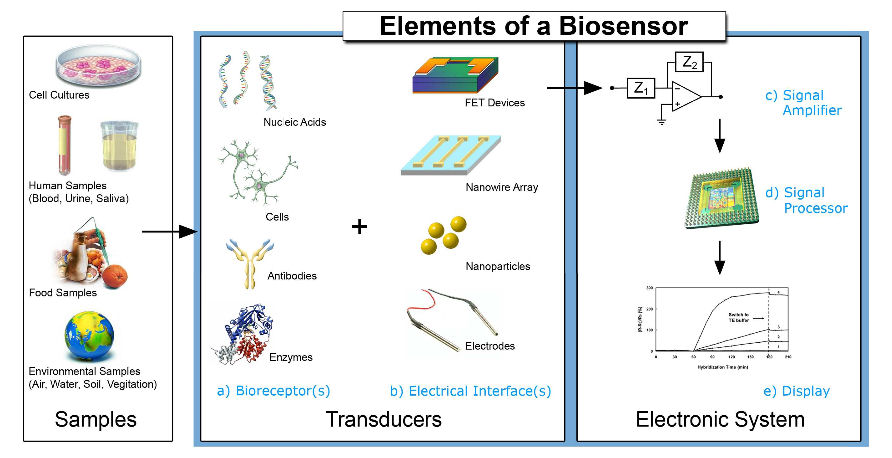
\includegraphics[width=3.5in]{Biosensor_System}
	\caption{General Bioelectronics Flow \cite{wiki:Biosensor_image}}
	\label{fig:flow}
\end{figure}
The arsenic detecting bioreceptor is able to sense the presence of arsenic in a
solution and affect the pH of another (?) solution. The pH is currently being
read by a simple (I assume) litmus test.
% needed in second column of first page if using \IEEEpubid
%\IEEEpubidadjcol

\subsection{Experiment}

The initial goal of the experiment is to convert an input signal, in this case
the presence of arsenic in solution, to an electrical signal. This goal
involves two steps, the first of which is to use a biological sensor to convert
the input signal into a format that can be read by an electrical transducer.
The chosen format involved the modulation of a solution's pH based on the
level of arsenic in solution. The biological sensor involved a \textbf{explain
genetic circuit}. After correlating the input signal with pH, the next step is
to convert pH into an electrical signal using a pH probe 
The basic elements involved in the experiment involve an input signal (arsenic
in solution) invoking an electrical response. This electrical response could be
processed by a microcontroller, after which there are many directions to go. 

\subsection{Design Elements}

Explain the different elements that will be involved in this complete circuit.

\subsubsection{Biosensor}

Explain who made the Biosensor and how it is currently being used. It will be
important to include the arsenic to pH curve.

\subsubsection{Silicon Nanowire}

Explain the background of the silicon nanowire. It will be important to include
the IV curve as well as the pH to current (assuming you are sweeping the Vsol)
and the pH to Vsol (assuming a constant drain current)

\subsection{Integration}

\subsubsection{Solution to Cell}

\subsubsection{Cell to pH}

\subsubsection{pH to Silicon Nanowire}

\subsubsection{Silicon Nanowire to EE (Voltage/Current)}

\subsubsection{EE (Voltage/Current) to A/D}

\subsubsection{A/D to Display}

% An example of a floating figure using the graphicx package.
% Note that \label must occur AFTER (or within) \caption.
% For figures, \caption should occur after the \includegraphics.
% Note that IEEEtran v1.7 and later has special internal code that
% is designed to preserve the operation of \label within \caption
% even when the captionsoff option is in effect. However, because
% of issues like this, it may be the safest practice to put all your
% \label just after \caption rather than within \caption{}.
%
% Reminder: the "draftcls" or "draftclsnofoot", not "draft", class
% option should be used if it is desired that the figures are to be
% displayed while in draft mode.
%
%\begin{figure}[!t]
%\centering
%\includegraphics[width=2.5in]{myfigure}
% where an .eps filename suffix will be assumed under latex, 
% and a .pdf suffix will be assumed for pdflatex; or what has been declared
% via \DeclareGraphicsExtensions.
%\caption{Simulation Results.}
%\label{fig_sim}
%\end{figure}

% Note that IEEE typically puts floats only at the top, even when this
% results in a large percentage of a column being occupied by floats.
% However, the Computer Society has been known to put floats at the bottom.


% An example of a double column floating figure using two subfigures.
% (The subfig.sty package must be loaded for this to work.)
% The subfigure \label commands are set within each subfloat command,
% and the \label for the overall figure must come after \caption.
% \hfil is used as a separator to get equal spacing.
% Watch out that the combined width of all the subfigures on a 
% line do not exceed the text width or a line break will occur.
%
%\begin{figure*}[!t]
%\centering
%\subfloat[Case I]{\includegraphics[width=2.5in]{box}%
%\label{fig_first_case}}
%\hfil
%\subfloat[Case II]{\includegraphics[width=2.5in]{box}%
%\label{fig_second_case}}
%\caption{Simulation results.}
%\label{fig_sim}
%\end{figure*}
%
% Note that often IEEE papers with subfigures do not employ subfigure
% captions (using the optional argument to \subfloat[]), but instead will
% reference/describe all of them (a), (b), etc., within the main caption.


% An example of a floating table. Note that, for IEEE style tables, the 
% \caption command should come BEFORE the table. Table text will default to
% \footnotesize as IEEE normally uses this smaller font for tables.
% The \label must come after \caption as always.
%
%\begin{table}[!t]
%% increase table row spacing, adjust to taste
%\renewcommand{\arraystretch}{1.3}
% if using array.sty, it might be a good idea to tweak the value of
% \extrarowheight as needed to properly center the text within the cells
%\caption{An Example of a Table}
%\label{table_example}
%\centering
%% Some packages, such as MDW tools, offer better commands for making tables
%% than the plain LaTeX2e tabular which is used here.
%\begin{tabular}{|c||c|}
%\hline
%One & Two\\
%\hline
%Three & Four\\
%\hline
%\end{tabular}
%\end{table}


% Note that IEEE does not put floats in the very first column - or typically
% anywhere on the first page for that matter. Also, in-text middle ("here")
% positioning is not used. Most IEEE journals use top floats exclusively.
% However, Computer Society journals sometimes do use bottom floats - bear
% this in mind when choosing appropriate optional arguments for the
% figure/table environments.
% Note that, LaTeX2e, unlike IEEE journals, places footnotes above bottom
% floats. This can be corrected via the \fnbelowfloat command of the
% stfloats package.








% if have a single appendix:
%\appendix[Proof of the Zonklar Equations]
% or
%\appendix  % for no appendix heading
% do not use \section anymore after \appendix, only \section*
% is possibly needed

% use appendices with more than one appendix
% then use \section to start each appendix
% you must declare a \section before using any
% \subsection or using \label (\appendices by itself
% starts a section numbered zero.)
%


\appendices
\section{Summary of Claimed Characteristics}
\subsection{Biosensor}
\subsection{Silicon Nanowire}
% you can choose not to have a title for an appendix
% if you want by leaving the argument blank
\section{Summary of Experimental Characteristics}
\subsection{Biosensor}
\subsection{Silicon Nanowire HIPPO}

% Can use something like this to put references on a page
% by themselves when using endfloat and the captionsoff option.
\ifCLASSOPTIONcaptionsoff
  \newpage
\fi



% trigger a \newpage just before the given reference
% number - used to balance the columns on the last page
% adjust value as needed - may need to be readjusted if
% the document is modified later
%\IEEEtriggeratref{8}
% The "triggered" command can be changed if desired:
%\IEEEtriggercmd{\enlargethispage{-5in}}

% references section

% can use a bibliography generated by BibTeX as a .bbl file
% BibTeX documentation can be easily obtained at:
% http://www.ctan.org/tex-archive/biblio/bibtex/contrib/doc/
% The IEEEtran BibTeX style support page is at:
% http://www.michaelshell.org/tex/ieeetran/bibtex/
\bibliographystyle{IEEEtran}
\bibliography{IEEEabrv,../bibtex_files/RPC.bib,../bibtex_files/Connecting_Ideas,../bibtex_files/Rethink_Toward_GP_uF_Chips,../bibtex_files/mf.bib,../bibtex_files/ece.bib,../bibtex_files/sb.bib}

%Bio Section
\begin{IEEEbiography}[{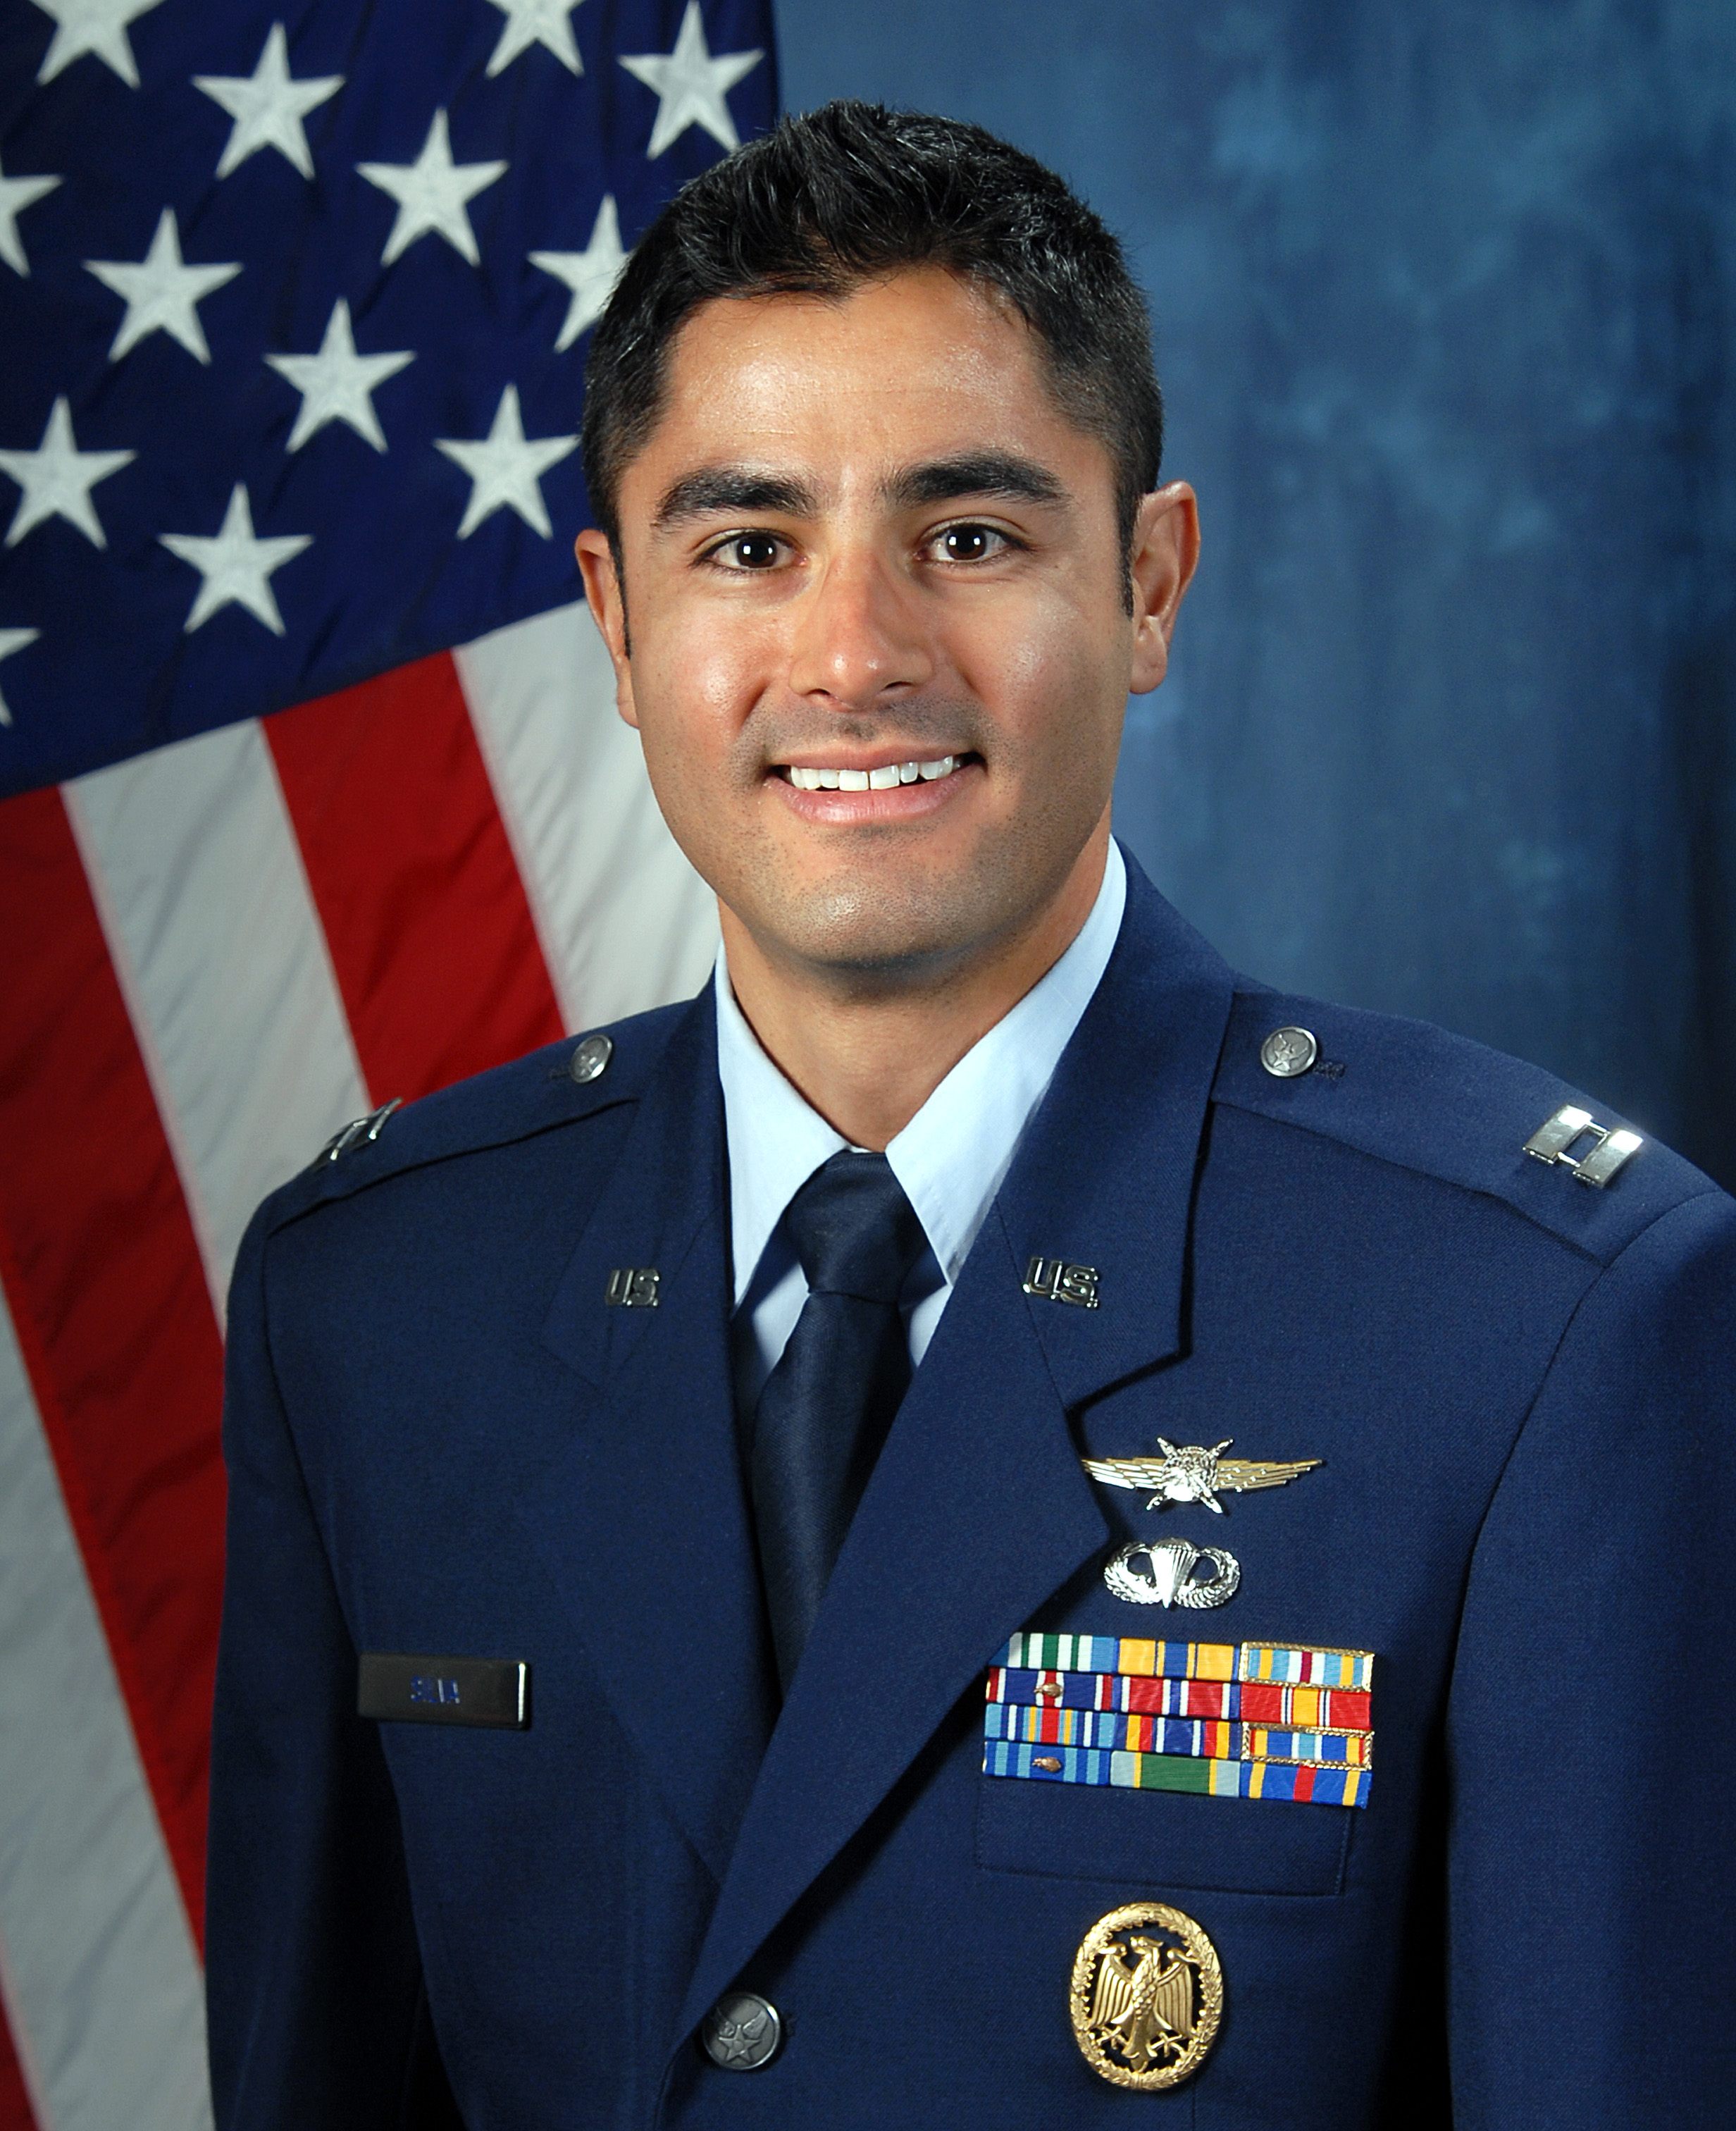
\includegraphics[width=1in,height=1.25in,clip,keepaspectratio]{silva_official_photo.jpg}}]{Ryan Silva}
% or if you just want to reserve a space for a photo:
%\begin{IEEEbiography}{Michael Shell}
%Biography text here.
	Ryan Silva is a Captain on active-duty in the United States Air Force.
	He is currently assigned to Boston University, where is pursuing his
	PhD in Computer Engineering. After graduating with his degree, Ryan
	will be assigned to an Air Force unit before returning to teach at the
	United States Air Force Academy, where he graduated with a degree in
	Electrical Engineering in 2005.
\end{IEEEbiography}
\end{document}

